\documentclass[a4paper,ngerman]{scrartcl}

\usepackage{amsmath}
\usepackage{amsfonts}
\usepackage{amssymb}
\usepackage[utf8]{inputenc}
\usepackage{graphicx}
\usepackage[ngerman]{babel}
\usepackage{hyperref}
\usepackage{float}
\usepackage{caption}
\usepackage{subcaption}
\usepackage{multirow}  %for tables
\usepackage{icomma} % Handle german comma as decimal point in numbers
\usepackage{units,siunitx} % Write units with correct spacing
\usepackage{upgreek} % provide non-italic greek letters
\usepackage{url}
\usepackage{booktabs}
\usepackage{hepnames}
%\usepackage{subfig}

% Formatting of table & figure captions
\captionsetup{font={sf,footnotesize},labelfont=bf,textfont=sl,skip=6pt}
\setlength{\abovecaptionskip}{6pt}
\setlength{\belowcaptionskip}{0pt}

%locale for units to german
\sisetup{locale = DE}
\sisetup{separate-uncertainty=true}

\title{Landéfaktor\\Versuchsauswertung}
\date{\today}
\author{Michel Rausch, Michael Eliachevitch}

\begin{document}

\maketitle
\tableofcontents
\newpage

\section{Zeitkalibrierung}

Ein Funktionsgenerator wurde an den Starteingang des TAC geschlossen, sowie über Verzögerungsglieder an den Stoppeingang. Diese wurden zugeschaltet, um die Zeitverzögerung in bekannten Schritten von \SI{1}{\micro\second} zu erhöhen. Die zugehörigen Peaks waren scharf gegenüber dem Abstand, sodass die Messungen sich in einer einzelnen Grafik, Abb. \ref{fig:zeitkalibrierung_hist}, auswerten ließen. Die Nummer des Kanals steigt mit der zugehörigen Verzögerung. 

\begin{figure}[tb!]
\centering
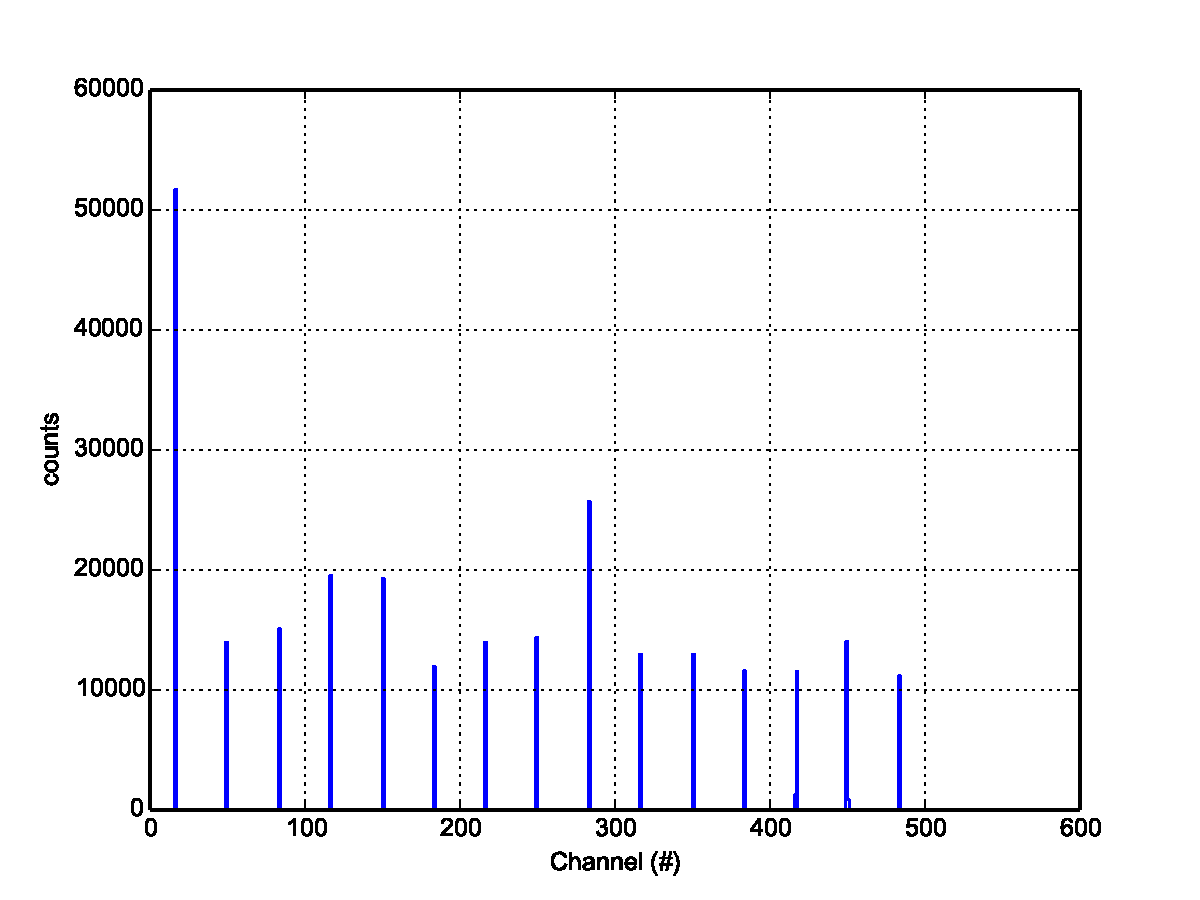
\includegraphics[width=0.7\textwidth]{abbildungen/zeitkalibrierung_hist.pdf}
\caption[Daten zur Zeitkalibrierung]{\textbf{Daten zur Zeitkalibrierung.} Die gezeigten Peaks gehören zu unterschiedlichen Verzögerungen. Die zugehörigen Peaks waren scharf gegenüber dem Abstand, sodass die Messungen in einer einzelnen Grafik auswerten ließen. Die Verzögerung wird von dem Peak am weitesten links nach rechts schrittweise um \SI{1}{\micro\second} größer.}
\label{fig:zeitkalibrierung_hist}
\end{figure}


Mittels des Python-Moduls \emph{numpy} wurde eine lineare Regression durchgeführt. Mit der resultierenden Geradengleichung wurden die Kanäle jeweils einer Zeit zugewiesen. Die Regression ist in Abbildung \ref{fig:zeitkalibrierung} gezeigt, das Ergebnis lautet

\begin{equation}
\label{eqn:Zeitkalibrierung}
\frac{\mathrm{Zeit}}{\mathrm{Kanal}} = \SI{29.9783924  +-  0.0000004 }{\nano\second} ~.
\end{equation}

Der Fehler der Zeitkalibrierung ist im Vergleich zu den anderen
Fehlern vernachlässigbar klein und wird im folgenden daher nicht
weiter fortgepflanzt.

\begin{figure}[tb!]
\centering
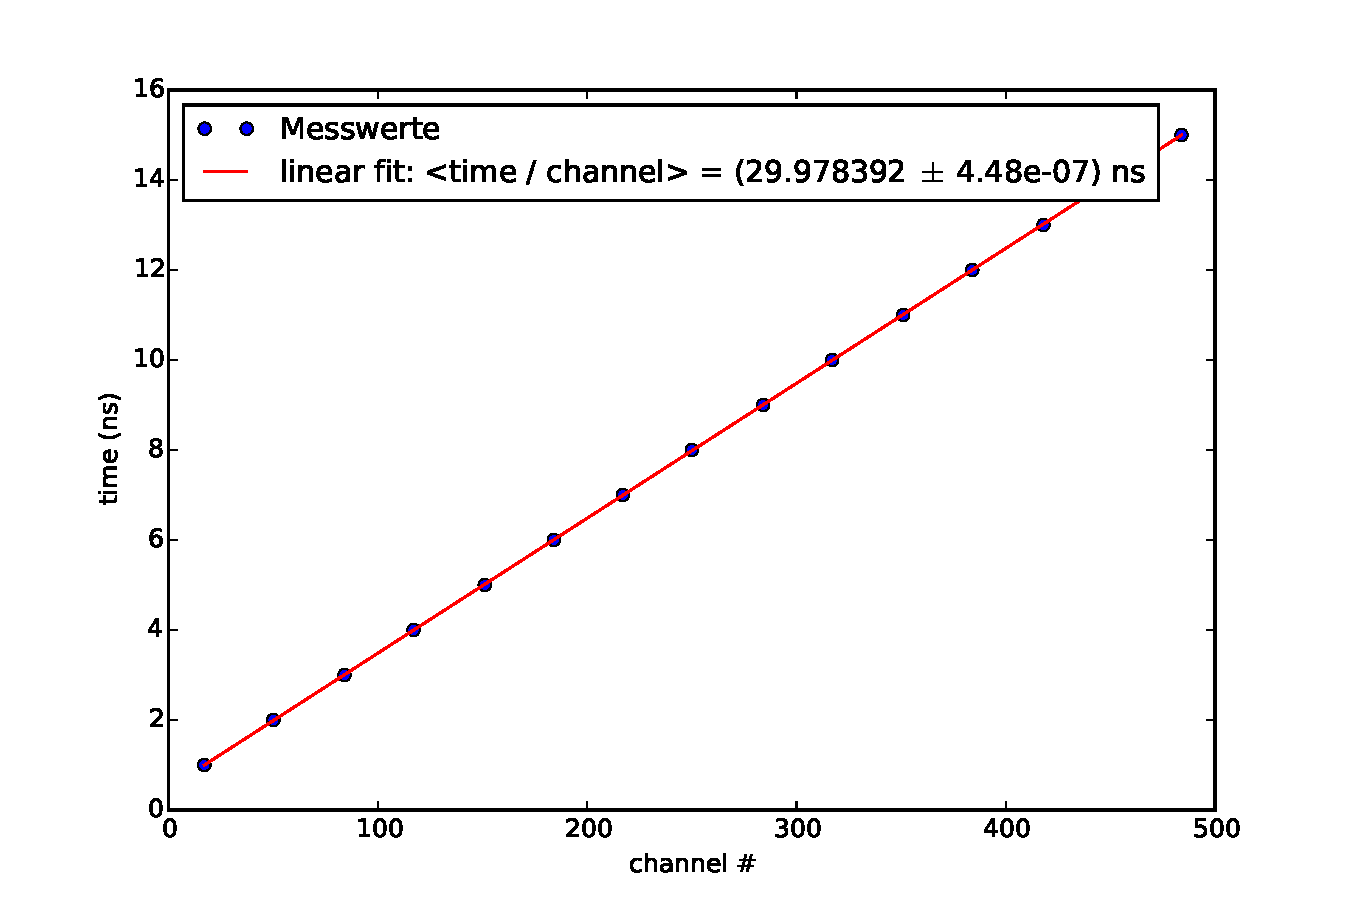
\includegraphics[width=0.7\textwidth]{abbildungen/zeitkalibrierung.pdf}
\caption[Zeitkalibrierung]{\textbf{Zeitkalibrierung.} Mittels eines Pythonscripts wurde ein linearer Fit durchgeführt. Die Kanalnummer des VKAs wurde auf der x-Achse aufgetragen, die dazugehörige Verzögerung auf der y-Achse. Mit der Geradengleichung wurden Kanäle einer Zeit zugeordnet.}
\label{fig:zeitkalibrierung}
\end{figure}





\section{Magnetfeld}

Das Magnetfeld wurde mit einer Hallsonde bestimmt. Aus den Daten der Kalibrierung, die übernommen wurde, konnte die gemessene Spannung am Vorwiderstand $U_{\mathrm{VW}}$ in die Magnetfeldstärke umgerechnet werden. Zur Umrechnung wurde 

\begin{equation}
\label{eqn:B-gauss}
B \mathrm{/G} = -1,68946 + 0,30472 \cdot U_{\mathrm{VW}} \mathrm{/mV}
\end{equation}

verwendet. In der Spule ist das Magnetfeld inhomogen. Der Fehler für die Inhomogenität wurden aus der übernommenen Messreihe in Tabelle \ref{tab:fieldinhomogenities} ermittelt. Es sind die Spannungen an der Hallsonde aufgelistet. Diese stehen in einem linearen Verhältnis zu der Magnetfeldstärke, daher können die relativen Fehler übernommen werden. Der relative Fehler für jeweils vier Werte, also für jeden Punkt entlang der Spule, wurde bestimmt. Über diese wurde gemittelt, um den mittleren relativen Fehler zu bestimmen. Dieser war

\begin{equation}
\label{eqn:inhomogen_fehler}
\sigma_{\mathrm{B}} = 0,02 = 2 \% ~.
\end{equation}

Die Spannung am Vorwiderstand betrug

\begin{equation}
U_{\mathrm{VW}} = \SI{123,6}{\milli \volt} ~.
\end{equation}

Hieraus ergab Formel \eqref{eqn:B-gauss}, mit dem Fehler für die Inhomogenität aus Gleichung \eqref{eqn:inhomogen_fehler},
\begin{equation}
\label{eq:B}
B = \SI[separate-uncertainty=true]{36.0 \pm 0.7 }{G} ~.
\end{equation}

\begin{table}[tb!]
\centering
\caption[Inhomogenität des Magnetfelds der Spule]{\textbf{Inhomogenität des Magnetfelds der Spule} Um den relativen Fehler zum Magnetfeld zu finden wurde auf vorliegende Messungen einer Hallsonde zurückgegriffen. Über verschiedene Punkte an der Länge $l$ der Spule wurde die Spannung an der Hallsonde gemessen. Für jeden dieser Punkte wurden vier Messwerte für verschiedene Positionen innerhalb des Spulenquerschnitts aufgenommen. Die mit "'*"' markierten Werte für $l = \SI{0.00}{m}$ und $l = \SI{1.00}{m}$ wischen stark von den anderen Werten ab, wurden daher nicht in die Berechnung des Fehlers aufgenommen.}
\begin{tabular}{ccccc}
\toprule 
$l$/m	&	$U_{\mathrm{Hall}} (0 \mathrm{m})$/mV	&	$U_{\mathrm{Hall}} (0,28 \mathrm{m})$/mV	&	$U_{\mathrm{Hall}}(- 0,28 \mathrm{m})$/mV	&	$U_{\mathrm{Hall}} (0 \mathrm{m})$/mV	\\
\midrule
0,00* & 149,6* & 123,6* & 123,6* & 139,7* \\
0,05 & 213,9 & 231,2 & 227,5 & 218,8 \\
0,10 & 243,6 & 257,1 & 257,2 & 243,6 \\
0,15 & 247,3 & 267,0 & 267,0 & 248,5 \\
0,20 & 253,4 & 271,0 & 272,0 & 249,7 \\
0,25 & 272,0 & 279,4 & 279,4 & 262,1 \\
0,30 & 288,1 & 284,3 & 285,6 & 291,8 \\
0,35 & 283,1 & 283,1 & 284,3 & 284,3 \\
0,40 & 270,7 & 279,4 & 281,9 & 270,7 \\
0,45 & 269,5 & 279,4 & 280,6 & 269,5 \\
0,50 & 279,4 & 280,6 & 283,1 & 278,2 \\
0,55 & 289,3 & 283,1 & 285,6 & 290,5 \\
0,60 & 289,3 & 284,3 & 285,6 & 289,3 \\
0,65 & 264,6 & 278,2 & 278,2 & 260,9 \\
0,70 & 273,2 & 279,4 & 280,6 & 273,2 \\
0,75 & 270,7 & 280,6 & 280,6 & 274,5 \\
0,80 & 259,6 & 274,5 & 274,5 & 257,2 \\
0,85 & 255,9 & 272,0 & 270,7 & 257,2 \\
0,90 & 243,6 & 262,1 & 260,9 & 244,8 \\
0,95 & 217,6 & 238,6 & 237,4 & 222,5 \\
1,00* & 157,0* & 160,7* & 155,8* & 163,2* \\
\bottomrule
\end{tabular}
\label{tab:fieldinhomogenities}
\end{table}


\clearpage
\section{Bestimmung der Lebensdauer des Myons}

Gemäß dem in der Vorbereitung in Abschnitt~3 besprochenen und in
Abbildung~2 gezeigtem Versuchsaufbau wurde die Lebensdauer der Myonen
gemessen. Gemessen wurde die Zeit zwischen dem Triggersignal obersten
Szintillator und dem Signal aus dem Myonzerfall, welches durch dabei
emittierte Positron ausgelöst wurde. Es wurden nur solche Ereignisse
selektiert, bei denen das Positron nach oben emittiert wurde, sodass
wir mit dem angelegten Magnetfeld eine Modulation erhalten, die der
Präzession des Myons im Magnetfeld entspricht.

Um eine für die Auswertung ausreichende Statistik zu erreichen, ist
bei der in unserem Aufbau verwendeten sensitiven Detektionsfläche von
$\approx \SI{1}{\square\meter}$ und dem kleinen Phasenraum der Messung eine
lange Messzeit von mehreren Tagen oder Wochen notwendig, um eine
ausreichende Statistik zu erhalten. Daher haben wir bereits vorhandene
Messwerte verwendet.

Diese wurden mit dem Analyse-Framework ROOT histogrammiert, wie in
Abbildung~\ref{fig:zerfallszeiten} zu sehen ist. Diese wurden dann mit
Gleichung~21 aus der Vorbereitung gefittet. Zur Erinnerung ist sie
hier noch einmal aufgeführt.

\begin{equation}
\label{eq:fitfkt}
N(t) = K \cdot \exp(- \frac{t}{\tau}) \cdot \left[ 1 + \overline{A} \cdot \cos(\omega t + \delta) \right] .
\end{equation}



Zur ermittlung der Startwerte wurde mit ROOT zuerst ein exponentieller
Fit ohne Modulation mit der Gleichung 
\begin{equation}
N(t) = K \cdot \exp(- \frac{t}{\tau})   
\end{equation}
durchgeführt und die Ergebnisse davon wurden als Startparameter für
den vollständtigen Fit mit Gleichung~\ref{eq:fitfkt} verwendet. Den
Startparameter für die Präzessionsfrequenz $\omega$ haben wir aus
einem aus der Quantenmechanik angenommenen Landéfaktor von $g = 2$
berechnet und erhielten

\begin{equation}
  \omega_{\rm LIT} = \frac{g \mu_{B}}{\hbar B} \approx \SI{6.3e8}{\per\second}~.
\end{equation}

Als Startparameter für die Phase wurde $\delta = 0$ gewählt. 
Für den Fit wurden nur die Einträge in den Kanälen 7 bist 500
verwendet, da erst ab Kanal 7 die Binhöhen anfangen zu sinken und nach
Kanal 500 alle Einträge bei 0 oder 1 liegen. Es wurde die Fit-Methode
des Histogramms verwendet. 

Aus dem Fit erhielten wir einen die effektive Lebensdauer 
\begin{equation}
\tau_{\rm eff} = \left(\SI{69,31}{} \pm \SI{0,61}{}\right)\,\textrm{Kanäle}~,
\end{equation}
beziehungsweise mit der Zeitkalibrierung aus Gleichung~\ref{eqn:Zeitkalibrierung}

\begin{equation}
\label{eq:tau}
\tau_{\rm eff} = \SI{2.08 +- 0.02}{\micro\second}~.
\end{equation}

% (mapcar (lambda (x) (* x  29.9783924)) '(6.93071e+01 6.09872e-01))

\begin{figure}[tbh!]
  \centering
  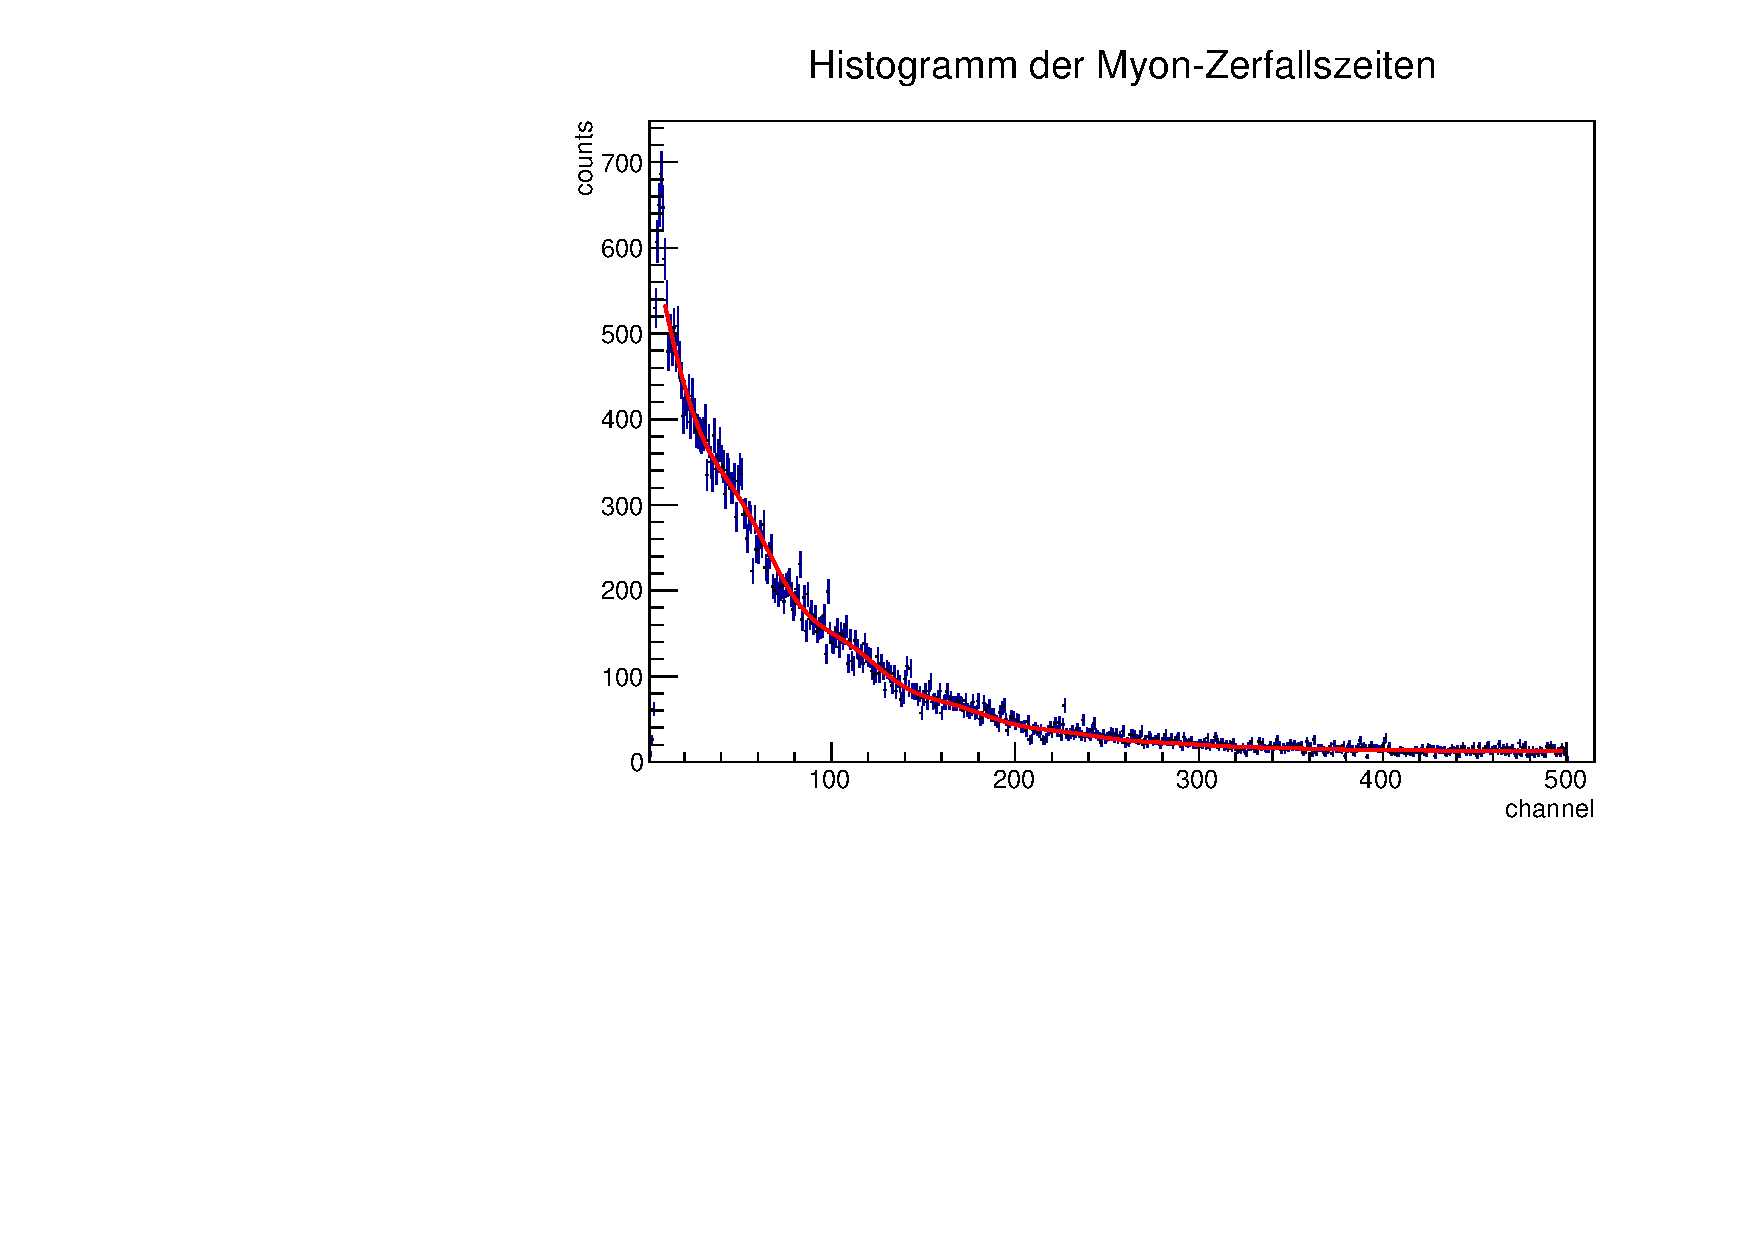
\includegraphics[width=\textwidth]{abbildungen/histogramm.pdf}
  \caption{\textbf{Histogramm der Myon-Zerfallszeiten}
  Eingetragen sind die Zeiten zwischen den Triggersignalen des oberen Szintillators und den
  Signalen aus dem Positron des \APmuon-Zefalls. Die Zeit ist dabei in Kanälen
  aufgetragen und kann nach Gleichung~\ref{eqn:Zeitkalibrierung} in
  Sekunden umgerechnet werden. Zu sehen ist ein exponentieller
  Abfall, wie es bei einem statistischen Prozess zu
  erwarten ist. Zusätzlich kommt es noch zu einer periodischen
  Modulation, da wir nur die Ereignisse selektiert haben, bei denen
  das Positron nach oben emittiert wurde und gleichzeitig ein Magnetfeld angelegt
  hatten. Das Myon emittiert das Positron bevorzugt in Spinrichtung
  und durch die Präzession im Magnetfeld kommt es zur sichtbaren
  Modulation. Damit kann die Präzessionsfrequenz und schließlich der
  Landéfaktor bestimmt werden.}

  \label{fig:zerfallszeiten}
\end{figure}

\clearpage
\section{Bedeutung des Landéfaktors}

Der Landéfaktor $g$ gibt für ein Teilchen das Verhältnis des gemessenen magnetischen Moments $ u_{\mathrm{gemessen}}$ zu dem klassisch erwartetem magnetischem Moment $u_{\mathrm{klassisch}}$ an. Demnach gilt

\begin{equation}
g = \frac{ u_{\mathrm{gemessen}} }{u_{\mathrm{klassisch}} } ~.
\end{equation}

Jeder Drehimpuls besitzt in einem Magnetfeld ein magnetisches Moment. Für unterschiedliche Drehimpulse können die Landéfaktoren voneinander abweichen. So ist $g$ für den Bahndrehimpuls eines geladenes Teilchens genau eins, für dessen Spin jedoch $2 + \text{Korrekturen höherer Ordnung}$. Auch negative Werte sind möglich. In einem Magnetfeld mit Betrag $B$ gilt mit der Präzessionsfrequenz $\omega$ und dem Bohrschem Magneton $\mu_\mathrm{B}$

\begin{equation}
g = \frac{\hbar \omega}{\mu_\mathrm{B} B} ~.
\end{equation}

\section{Bestimmung des Landéfaktors des Myons}
Aus dem Fit in Abbildung~\ref{fig:zerfallszeiten} der Zerfallszeiten
erhielten wir neben dem Landéfaktor die Präzessionsfrequenz
der Myonen, die mit der Zeitkalibrierung in
Gleichung~\ref{eqn:Zeitkalibrierung}

\begin{equation}
\label{eq:omega}
% (mapcar (lambda (x) (* x  29.9783924)) '(1.70217e-02   3.56301e-04  ))
\omega = \SI{0.510 +-  0.011}{\per\nano\second}
\end{equation}
beträgt. Daraus erhält man den Landéfaktor

% (setq mub 9.27401e-24)
% (setq hbar 1.05457173e-34)
% (setf B 36e-4)
% (setf omega 0.51e9)
% (* (/ hbar mub) (/ omega B)

\begin{equation}
g = \frac{\hbar \omega}{\mu_B B} = \SI{1.611}{}~.
\end{equation}

Es fehlt noch die Fehlerabschätzung. Da sich der Fehler auf die
Präzessionsfrequenz und auf das Magnetfeld nur multiplikativ auf das
Endergebnis auswirken, bleiben die relativen Fehler erhalten. Aus den
Gleichungen \ref{eqn:inhomogen_fehler} und \ref{eq:omega} erhalten wir

\begin{equation}
  \begin{split}
    \sigma_B &= 2\%\\
    \sigma_{\omega} &= \frac{\SI{0,011}{}}{\SI{0,51}{}} = 2\%~.\\
  \end{split}
\end{equation}

%(* 0.02 1.611) 0.03222
Damit haben der statistische Fehler aus dem Fit der Präzessionsfrequenz
$\sigma_{\omega}$ und der systematische Fehler $\sigma_B$ aus dem
Magnetfeld den selben absoluten Wert 0,03 und wir erhalten somit

\begin{equation}
  \label{eq:g}
    g = \SI{1.61}{} \pm \SI{0.03}{} \pm \SI{0.03}{}~.
\end{equation}


\clearpage

\section{Diskussion der Ergebnisse}
Unser Ergebnis für die Lebensdauer von Myonen von 
$\tau_{\rm eff} = \SI{2.08 +- 0.02}{\micro\second}$\eqref{eq:tau}
ist sehr zufriedenstellend. Sie liegt damit zwar unter dem
Literaturwert für die Lebensdauer von freien Myonen, der bei 
\SI{2.197}{\micro\second} liegt [\ref{ref:pdg14}], was jedoch daran
liegt, dass wir die effektive Lebensdauer in einem Material gemessen
haben, welche etwas niedriger ist. Bei Zeiten unter
\SI{1}{\micro\second} spielt noch der Zerfall von negativen Myonen in
Elektronen eine Rolle, welcher aufgrund eines zusätzlichen
Zerfallskanals im Kern eine deutlich niedrigere Zeitkonstante hat,
aber womöglich haben selbst positive Myonen im Material eine etwas
niedrigere Lebensdauer als im Vakuum.\\

Der gemessene Landéfaktor von $g = \SI{1.61}{} \pm \SI{0.03}{} \pm
\SI{0.03}{}$~\eqref{eq:g} unterscheidet sich deutlich von dem
theoretisch erwartenen Landéfaktor für Myonen von $g = 2$ und die
Differenz liegt auch deutlich außerhalb unserer Fehlergrenzen. Eine
möglicher Grund ist ein systematischer Feler auf das Magnetfeld, der
größer ist, als unsere Fehlerrechnung es ergeben hat. Ein anderen
Grund könnte ein Fehler in der Modulation $\omega$ sein, da deren
Amplitude sehr gering ist. Womöglich treten aber auch hier Störeffekte
auf, da der Landéfaktor in einem Matierial gemessen wurde.




\section{Quellen}
\begin{enumerate}
\item Vorbereitungsmappe 
\item \emph{Einführung in das Kernphysikalische Praktikum} von F. K. Schmidt, 
  Überarbeitung von J. Wolf, Ausgabe September 2009. \label{ref:bb}
\item K.A. Olive et al. (Particle Data Group), Chin. Phys. C, 38, 090001 (2014). \label{ref:pdg14}
\end{enumerate}



\end{document}
